%%
%% This is file `sample-sigconf-authordraft.tex',
%% generated with the docstrip utility.
%%
%% The original source files were:
%%
%% samples.dtx  (with options: `all,proceedings,bibtex,authordraft')
%% 
%% IMPORTANT NOTICE:
%% 
%% For the copyright see the source file.
%% 
%% Any modified versions of this file must be renamed
%% with new filenames distinct from sample-sigconf-authordraft.tex.
%% 
%% For distribution of the original source see the terms
%% for copying and modification in the file samples.dtx.
%% 
%% This generated file may be distributed as long as the
%% original source files, as listed above, are part of the
%% same distribution. (The sources need not necessarily be
%% in the same archive or directory.)
%%
%%
%% Commands for TeXCount
%TC:macro \cite [option:text,text]
%TC:macro \citep [option:text,text]
%TC:macro \citet [option:text,text]
%TC:envir table 0 1
%TC:envir table* 0 1
%TC:envir tabular [ignore] word
%TC:envir displaymath 0 word
%TC:envir math 0 word
%TC:envir comment 0 0
%%
%% The first command in your LaTeX source must be the \documentclass
%% command.
%%
%% For submission and review of your manuscript please change the
%% command to \documentclass[manuscript, screen, review]{acmart}.
%%
%% When submitting camera ready or to TAPS, please change the command
%% to \documentclass[sigconf]{acmart} or whichever template is required
%% for your publication.
%%
%%

\documentclass[sigconf,language=spanish]{acmart}
%\documentclass[sigconf,language=spanish]{acmart}
%%
%% \BibTeX command to typeset BibTeX logo in the docs
\AtBeginDocument{%
  \providecommand\BibTeX{{%
    Bib\TeX}}}

%% Rights management information.  This information is sent to you
%% when you complete the rights form.  These commands have SAMPLE
%% values in them; it is your responsibility as an author to replace
%% the commands and values with those provided to you when you
%% complete the rights form.
\setcopyright{acmlicensed}
\copyrightyear{2025}
\acmYear{2025}
\acmDOI{XXXXXXX.XXXXXXX}
%% These commands are for a PROCEEDINGS abstract or paper.
\acmConference[PCIC: GENAI '25]{Modelos Generativos Profundos}{2026-I}{Ciudad de México, México}
%%
%%  Uncomment \acmBooktitle if the title of the proceedings is different
%%  from ``Proceedings of ...''!
%%
%%\acmBooktitle{Woodstock '18: ACM Symposium on Neural Gaze Detection,
%%  June 03--05, 2018, Woodstock, NY}
%\acmISBN{978-1-4503-XXXX-X/2025/06}


%%
%% Submission ID.
%% Use this when submitting an article to a sponsored event. You'll
%% receive a unique submission ID from the organizers
%% of the event, and this ID should be used as the parameter to this command.
%%\acmSubmissionID{123-A56-BU3}

%%
%% For managing citations, it is recommended to use bibliography
%% files in BibTeX format.
%%
%% You can then either use BibTeX with the ACM-Reference-Format style,
%% or BibLaTeX with the acmnumeric or acmauthoryear sytles, that include
%% support for advanced citation of software artefact from the
%% biblatex-software package, also separately available on CTAN.
%%
%% Look at the sample-*-biblatex.tex files for templates showcasing
%% the biblatex styles.
%%

%%
%% The majority of ACM publications use numbered citations and
%% references.  The command \citestyle{authoryear} switches to the
%% "author year" style.
%%
%% If you are preparing content for an event
%% sponsored by ACM SIGGRAPH, you must use the "author year" style of
%% citations and references.
%% Uncommenting
%% the next command will enable that style.
%%\citestyle{acmauthoryear}

\usepackage{svg}
%%
%% end of the preamble, start of the body of the document source.
\begin{document}

%%
%% The "title" command has an optional parameter,
%% allowing the author to define a "short title" to be used in page headers.
\title{Music Transformer: Generación Automática de Música Monofónica al estilo de J.S. Bach Usando Transformers}

%%
%% The "author" command and its associated commands are used to define
%% the authors and their affiliations.
%% Of note is the shared affiliation of the first two authors, and the
%% "authornote" and "authornotemark" commands
%% used to denote shared contribution to the research.
\author{Rodrigo S. Cortez Madrigal}
%\authornote{Both authors contributed equally to this research.}
\email{rcortez@enesmorelia.unam.mx}
\orcid{0000-0003-4600-9644}
\authornotemark[1]
%\email{webmaster@marysville-ohio.com}
\affiliation{%
  \institution{PCIC}
  \city{CDMX}
  %\state{Ohio}
  \country{México}
}

%%
%% By default, the full list of authors will be used in the page
%% headers. Often, this list is too long, and will overlap
%% other information printed in the page headers. This command allows
%% the author to define a more concise list
%% of authors' names for this purpose.
%\renewcommand{\shortauthors}{Trovato et al.}

%%
%% The abstract is a short summary of the work to be presented in the
%% article.
\begin{abstract}

La composición musical es una forma de arte compleja, altamente creativa y hasta ahora inherentemente humana. Componer implica combinar distintos aspectos musicales como la melodía, la armonía, el ritmo e incluso otros no necesariamente musciales como la emoción, la cultura y la capacidad de innovar dentro de estructuras musicales establecidas. 
Esto hace de la generación automática de música un desafío significativo para los sistemas de inteligencia artificial y que ha sido un problema importante desde hace algunos años en el campo de la inteligencia artificial.
Los avances en modelos de lenguaje y arquitecturas de redes neuronales, como los Transformers, ha surgido un interés renovado en la capacidad de estas técnicas para generar música coherente y estilísticamente diversa.
En este trabajo, exploramos el uso de Transformers para la generación automática de música monofónica, evaluando su capacidad para producir piezas musicales que sean tanto coherentes como creativas.

\end{abstract}

%%
%% The code below is generated by the tool at http://dl.acm.org/ccs.cfm.
%% Please copy and paste the code instead of the example below.
%%
%\begin{CCSXML}
%<ccs2012>
% <concept>
%  <concept_id>00000000.0000000.0000000</concept_id>
%  <concept_desc>Do Not Use This Code, Generate the Correct Terms for Your Paper</concept_desc>
%  <concept_significance>500</concept_significance>
% </concept>
% <concept>
%  <concept_id>00000000.00000000.00000000</concept_id>
%  <concept_desc>Do Not Use This Code, Generate the Correct Terms for Your Paper</concept_desc>
%  <concept_significance>300</concept_significance>
% </concept>
% <concept>
%  <concept_id>00000000.00000000.00000000</concept_id>
%  <concept_desc>Do Not Use This Code, Generate the Correct Terms for Your Paper</concept_desc>
%  <concept_significance>100</concept_significance>
% </concept>
% <concept>
%  <concept_id>00000000.00000000.00000000</concept_id>
%  <concept_desc>Do Not Use This Code, Generate the Correct Terms for Your Paper</concept_desc>
%  <concept_significance>100</concept_significance>
% </concept>
%</ccs2012>
%\end{CCSXML}

%\ccsdesc[500]{Do Not Use This Code~Generate the Correct Terms for Your Paper}
%\ccsdesc[300]{Do Not Use This Code~Generate the Correct Terms for Your Paper}
%\ccsdesc{Do Not Use This Code~Generate the Correct Terms for Your Paper}
%\ccsdesc[100]{Do Not Use This Code~Generate the Correct Terms for Your Paper}

%%
%% Keywords. The author(s) should pick words that accurately describe
%% the work being presented. Separate the keywords with commas.
\keywords{Music Generation, Transformers, Deep Learning, Artificial Intelligence, Music Composition, Sequence Modeling, Bach Style}
%% A "teaser" image appears between the author and affiliation
%% information and the body of the document, and typically spans the
%% page.
\begin{teaserfigure}
  \includegraphics[width=\textwidth]{svg-inkscape/2000epochs.pdf}
  \caption{Pieza musical generada por el modelo Music Transformer entrenado por 2000 épocas.}
  \Description{Pieza musical generada por el modelo Music Transformer entrenado por 2000 épocas.}
  \label{fig:teaser}
\end{teaserfigure}

\received{20 February 2007}
\received[revised]{12 March 2009}
\received[accepted]{5 June 2009}

%%
%% This command processes the author and affiliation and title
%% information and builds the first part of the formatted document.
\maketitle

\section{Introduction}

\begin{quote}
Music is liquid architecture

\hfill--- Johann Wolfgang von Goethe
\end{quote}

La composición musical automática ha sido un área de investigación activa en inteligencia artificial durante varias décadas. 
El objetivo es desarrollar sistemas capaces de generar música que sea coherente, creativa y estilísticamente diversa, emulando la capacidad humana para componer música.
No obstante, la música es una forma de arte compleja que involucra múltiples dimensiones, incluyendo la melodía, la armonía, el ritmo y la estructura, lo que hace que la generación automática de música sea un desafío significativo. 
Además, la música está profundamente ligada a aspectos culturales y emocionales, lo que añade otra capa de complejidad al problema.

Sí bien se han explorado diversas técnicas para la generación automática de música, incluyendo modelos basados en reglas, redes neuronales recurrentes (RNNs) y modelos generativos adversariales (GANs), los avances recientes en modelos de lenguaje y arquitecturas de redes neuronales, como los Transformers, han abierto nuevas posibilidades para la generación de música.
Sin embargo, la generación de música implica dimensiones extras que no están presentes en el texto, como la armonía y el ritmo, lo que requiere adaptaciones específicas de estas arquitecturas para capturar las complejidades musicales. 
Mientras que en la generación de texto, se trabaja con un solo stream, la música puede ser polifónica, involucrando múltiples voces que interactúan entre sí. 
Además, la música tiene una estructura temporal más compleja, con patrones rítmicos y métricos que deben ser considerados y que no estan presentes en la generación de texto.

Para simplificar el problema, en este trabajo nos enfocamos en la generación de música monofónica, donde solo hay una línea melódica sin armonía o contrapunto. 
Con esta simplifiación podemos pensar en la música como una secuencia de eventos en el tiempo, podemos abordar la generación musical como un problema de predicción de secuencias. 
Esto nos permite centrarnos en la generación de secuencias de notas y duraciones, facilitando la aplicación de modelos basados en Transformers para este propósito. Los modelos de lenguaje basados en Transformers han demostrado un rendimiento sobresaliente en tareas de procesamiento del lenguaje natural, gracias a su capacidad para capturar dependencias a largo plazo y modelar contextos complejos. 
Estas características los hacen particularmente adecuados para la generación de música, donde las relaciones entre notas y frases necesariamente dependen de contextos amplios, es decir de todas las secuencias musicales anteriores.

\section{Antecedentes}

Anteriormente, se han utilizado diversas técnicas para la generación automática de música, incluyendo modelos basados en reglas, redes neuronales recurrentes (RNNs) y modelos generativos adversariales (GANs).
Los modelos basados en reglas dependen de conjuntos predefinidos de reglas musicales, lo que limita su capacidad para generar música novedosa y creativa, por ejemplo se han utilizado gramáticas formales para definir estructuras musicales o incluso algoritmos evolutivos para explorar espacios de composición.
Algoritmos que dependen en gran medida de las reglas musicales predifinidas o de las funciones objetivo que inherentemente limitan la creatividad y diversidad de la música generada y como sea requieren una considerable intervención humana para definir dichas reglas.

Los GANs han mostrado promesas en la generación de música, pero a menudo requieren un entrenamiento complejo y pueden ser difíciles de estabilizar. Redes como WaveGAN y MuseGAN han sido propuestas para generar audio y secuencias musicales, respectivamente, pero enfrentan desafíos en la coherencia a largo plazo y la calidad del audio generado.
Estas redes tiene un efoque generativo en el que a partir de la arquitectura de dos redes neuronales (generador y discriminador) se busca generar música que sea indistinguible de la música real, pero a menudo luchan por capturar la estructura musical a largo plazo. 
Esto implica tratar el audio como una imagen (espectrograma) y se genera toda la pieza musical de una sola vez, sin separar ni considerar las distintas capas musicales (melodía, armonía, ritmo, etc.).

En contratse a las GANs, los modelos autoregresivos generan música de manera secuencial, prediciendo cada nota o evento musical basado en los eventos anteriores. 
Aunque los modelos autoregresivos tradicionales, como las RNNs y LSTMs, han sido utilizados para la generación de música, enfrentan limitaciones en la captura de dependencias a largo plazo y en la modelación de contextos complejos.
Actualmente, los Transformers han superado a las RNNs en muchas tareas de secuencia a secuencia, gracias a su capacidad para modelar relaciones a largo plazo mediante mecanismos de atención.
Modelos como Music Transformer y MuseNet han demostrado la capacidad de los Transformers para generar música coherente y estilísticamente diversa, capturando estructuras musicales complejas y variaciones estilísticas.

\section{Objetivos}

- ¿Es posible entrenar un modelo Transformer para generar música monofónica al estilo de J. S. Bach?

- En este trabajo, exploramos el uso de Transformers para la generación automática de música, evaluando su capacidad para producir piezas musicales al estilo de J. S. Bach que sean coherentes y creativas.

\section{Metodología}

A través de la implentación de un decodificador Transformer, inspirado en MuseNet de OpenAI, que a la vez utiliza un decodificador Transformer (similar a GPT-3) entrenado para predecir la siguiente nota dada una secuencia de notas anteriores, se busca generar música monofónica al estilo de J. S. Bach.

El \textit{generative pre-trained transformer} (GPT) es un modelo de lenguaje autoregresivo basado en la arquitectura Transformer, presentado por OpenAI en en el paper \textit{Improving Language Understanding by Generative Pre-Training} \cite{radford_improving_2018} casi un año después de la publicación del paper \textit{Attention is all you need} \cite{vaswani_attention_2023} en el que se introdujo la arquitectura Transformer.
GPT se entrena en dos etapas: preentrenamiento y ajuste fino. Durante el preentrenamiento, el modelo se expone a una gran cantidad de texto no etiquetado y aprende a predecir la siguiente palabra en una secuencia dada su contexto previo. 
En la etapa de ajuste fino, el modelo se entrena en tareas específicas con conjuntos de datos etiquetados, adaptando sus conocimientos generales a tareas concretas como traducción, resumen o respuesta a preguntas.

Recordemos que el núcleo de la arquitectura Transformer es el mecanismo de atención, que permite al modelo enfocarse en diferentes partes de la secuencia de entrada al generar cada palabra.
Para entender los transformers, es importante comprender el concepto de \textit{self-attention} o atención propia, que permite al modelo evaluar la importancia relativa de cada palabra en la secuencia con respecto a las demás.
En un Transformer, cada palabra de la secuencia se representa mediante tres vectores: \text{query} (Q), \textit{key} (K) y \textit{value} (V). 
La atención se calcula utilizando estos vectores para determinar qué palabras son más relevantes para la predicción de la siguiente palabra.
El proceso de atención se realiza mediante el producto punto entre los vectores Q y K, seguido de una normalización softmax para obtener los pesos de atención. 
Estos pesos se utilizan luego para ponderar los vectores V, produciendo una representación contextualizada de la palabra actual en función de su relación con las demás palabras en la secuencia.

\begin{figure}[h]
  \centering
  \includegraphics[width=0.9\linewidth]{svg-inkscape/arch.png}
  \caption{Diagrama de la arquitectura del modelo Transformer}
  \label{fig:arquitectura-transformer}
\end{figure}

\subsection{Arquitectura del modelo}

Cada Transformer generador de texto consta de estos tres componentes clave:

Embedding: la entrada de texto se divide en unidades más pequeñas llamadas tokens, que pueden ser palabras o subpalabras. Estos tokens se convierten en vectores numéricos llamados incrustaciones, que capturan el significado semántico de las palabras.

Bloque Transformer: El componente fundamental del modelo que procesa y transforma los datos de entrada. Cada bloque incluye:

  Mecanismo de atención, el componente central del bloque Transformer. Permite que los tokens se comuniquen con otros tokens, capturando información contextual y relaciones entre palabras.

  Capa MLP (Multilayer Perceptron), una red de avance que opera en cada token de forma independiente. Mientras que el objetivo de la capa de atención es enrutar la información entre tokens, el objetivo de la MLP es refinar la representación de cada token.

Probabilidades de salida: Las capas lineales y softmax finales transforman las incrustaciones procesadas en probabilidades, lo que permite al modelo hacer predicciones sobre el siguiente token de una secuencia.

\subsubsection{Embedding}

El embedding es una representación densa y continua de las palabras o tokens en un espacio vectorial.
Cada palabra o token se asigna a un vector de números reales, donde la proximidad entre los vectores refleja la similitud semántica entre las palabras.
Esto permite que el modelo capture relaciones complejas entre palabras y mejore su capacidad para entender el contexto.

Para calcular el embedding, se utiliza una matriz de embedding que se aprende durante el entrenamiento del modelo.
Cada token de entrada se convierte en un índice que se utiliza para buscar su vector correspondiente en la matriz de embedding.
Además, se agrega una codificación posicional a los embeddings para proporcionar información sobre la posición de cada token en la secuencia, ya que los Transformers no tienen una estructura secuencial inherente como las RNNs.

Adicionalmente, tambien se utiliza el positional embedding, que es una técnica para incorporar información sobre la posición de las palabras en la secuencia.
Dado que los Transformers no tienen una estructura secuencial inherente, el positional encoding agrega información sobre la posición de cada token en la secuencia.
Esto se logra mediante la adición de vectores de codificación posicional a los embeddings de las palabras.
Estos vectores se calculan utilizando funciones trigonométricas (seno y coseno) de diferentes frecuencias, lo que permite al modelo distinguir entre diferentes posiciones en la secuencia.

\begin{figure}[h]
  \centering
  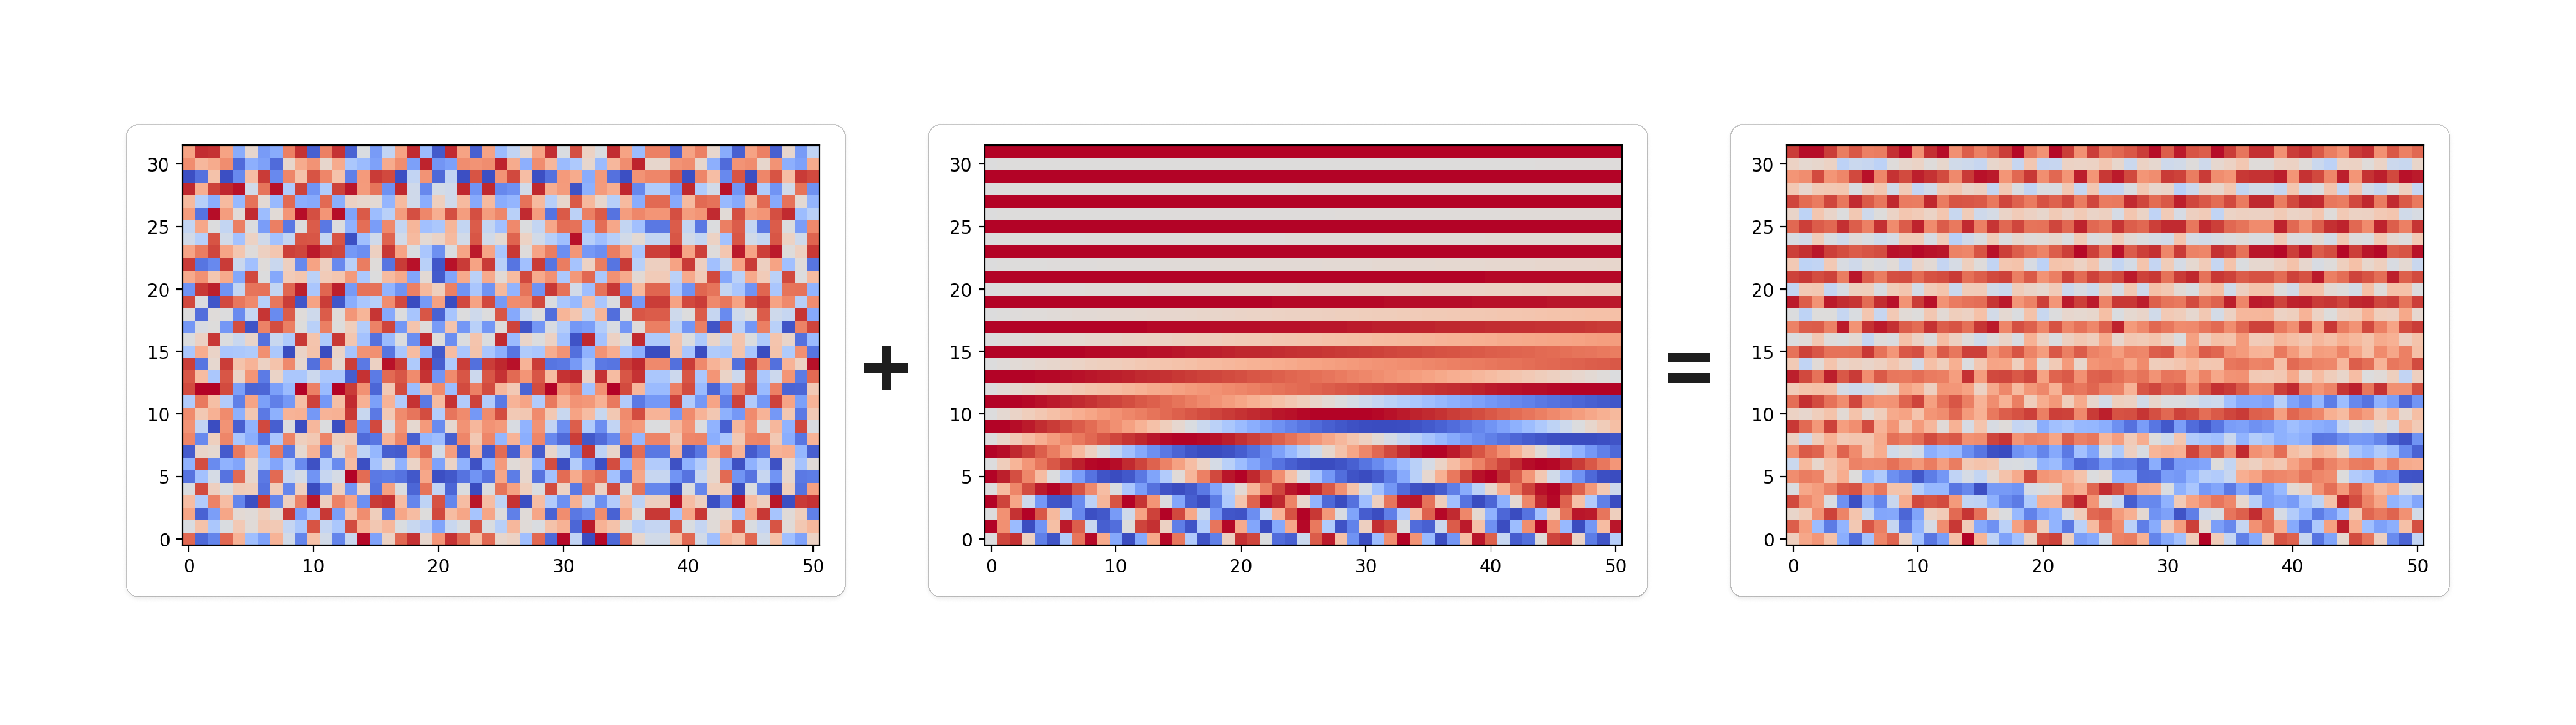
\includegraphics[width=1\linewidth]{svg-inkscape/embeddings.pdf}
  \caption{Representación de los embeddings y codificación posicional en el modelo Transformer.}
  \label{fig:embedding}
\end{figure}

La máscara de atención (attention mask) es un componente crucial en los modelos Transformer, especialmente en tareas de generación de texto.
Su función principal es controlar qué partes de la secuencia de entrada pueden ser atendidas por el modelo durante el proceso de atención.
En el contexto de la generación de texto, la máscara de atención se utiliza para evitar que el modelo "mire hacia adelante" en la secuencia, es decir, para asegurarse de que cada token solo pueda atender a los tokens anteriores en la secuencia y no a los futuros.
Esto es esencial para mantener la coherencia temporal y garantizar que las predicciones se basen únicamente en el contexto disponible hasta ese punto.

\subsubsection{Bloque Transformer}

El bloque Transformer consta de dos subcomponentes principales: el mecanismo de atención y la capa MLP (Multilayer Perceptron).

Mecanismo de atención: El mecanismo de atención permite que el modelo evalúe la importancia relativa de cada token en la secuencia con respecto a los demás.
Se calcula utilizando los vectores de consulta (Q), clave (K) y valor (V) para cada token.
El proceso de atención implica calcular el producto punto entre Q y K, seguido de una normalización softmax para obtener los pesos de atención.
Estos pesos se utilizan para ponderar los vectores V, produciendo una representación contextualizada de cada token.

Capa MLP: La capa MLP es una red de avance que opera en cada token de forma independiente.
Consta de dos capas lineales con una función de activación no lineal (como ReLU) entre ellas.
El objetivo de la capa MLP es refinar la representación de cada token, permitiendo al modelo capturar características más complejas y mejorar su capacidad para generar texto coherente.

\subsubsection{Probabilidades de salida}

Las capas lineales y softmax finales transforman las incrustaciones procesadas en probabilidades, lo que permite al modelo hacer predicciones sobre el siguiente token de una secuencia.

\subsubsection{Particularidades del modelo implementado}

El modelo (inspirado en MuseNet de OpenAI) implementado en este trabajo tiene las siguientes características específicas y fue tomado de \cite{foster_generative_2023}:

\begin{itemize}
    \item \textbf{Entradas dobles:} El modelo recibe dos secuencias de entrada, una para notas y otra para duraciones, lo que permite capturar tanto la melodía como el ritmo de la música.
    \item \textbf{Embeddings personalizados:} Se utilizan capas de embedding personalizadas para notas y duraciones, con dimensiones específicas para cada tipo de token.
    \item \textbf{Concatenación de embeddings:} Los embeddings de notas y duraciones se concatenan antes de ser procesados por el bloque Transformer, permitiendo al modelo considerar ambas características simultáneamente.
    \item \textbf{Bloque Transformer único:} El modelo utiliza un solo bloque Transformer para procesar la secuencia concatenada, simplificando la arquitectura y reduciendo la complejidad computacional.
    \item \textbf{Salidas duales:} El modelo tiene dos salidas separadas, una para predecir la siguiente nota y otra para predecir la duración, lo que permite una generación musical más precisa y controlada.
\end{itemize}

\begin{figure}[h]
  \centering
  \includegraphics[width=0.9\linewidth]{svg-inkscape/archconcat.png}
  \caption{Diagrama de la arquitectura del modelo Transformer}
  \label{fig:arquitectura-transformer}
\end{figure}

\subsection{Implementación}

El modelo implementado es una red neuronal basada en la arquitectura Transformer, diseñada para la generación de música monofónica. Su estructura es la siguiente:

\begin{itemize}
    \item \textbf{Entradas:} El modelo recibe dos secuencias de entrada, una para notas (\texttt{input\_layer}) y otra para duraciones (\texttt{input\_layer\_1}), ambas de longitud variable.
    \item \textbf{Embeddings:} Cada entrada pasa por una capa de embedding personalizada (\texttt{TokenAndPositionEmbedding}), que transforma los tokens en vectores de dimensión 128 e incorpora información posicional. La capa de notas tiene 7,552 parámetros y la de duraciones 3,072.
    \item \textbf{Concatenación:} Los embeddings de notas y duraciones se concatenan a lo largo de la dimensión de características, formando una secuencia de vectores de tamaño 256.
    \item \textbf{Bloque Transformer:} La secuencia concatenada se procesa mediante un bloque Transformer (\texttt{TransformerBlock}) con atención multi-cabeza, que permite capturar dependencias a largo plazo en la secuencia musical. Este bloque es el componente más pesado del modelo, con 1,447,424 parámetros.
    \item \textbf{Salidas:} La salida del Transformer se bifurca en dos capas densas:
    \begin{itemize}
        \item \texttt{note\_outputs}: predice la siguiente nota, con una capa densa de 59 unidades (15,163 parámetros).
        \item \texttt{duration\_outputs}: predice la duración, con una capa densa de 24 unidades (6,168 parámetros).
    \end{itemize}
    \item \textbf{Parámetros:} El modelo tiene un total de 1,479,379 parámetros, todos entrenables.
\end{itemize}

Esta arquitectura permite al modelo predecir, en cada paso de la secuencia, tanto la nota como la duración siguiente, utilizando el contexto musical previo gracias al mecanismo de atención del Transformer.

\subsection{Conjunto de Datos}

El conjunto de datos utilizado para entrenar el modelo Transformer consistió en un conjunto pequeño 
de archivos MIDI de música clásica de Bach descargados de http://www.jsbach.net.

\subsubsection{SMF: Standard MIDI File}

No confundir con MIDI, que es un protocolo de comunicación entre instrumentos musicales electrónicos.

Un SMF es un archivo que sigue el estándar MIDI para almacenar estas instrucciones musicales, es decir, notas, ritmo y tempo, en lugar de datos de audio. Los archivos SMF son ampliamente utilizados en la producción musical, la composición y la educación musical debido a su capacidad para representar música de manera compacta y flexible.

Los archivos MIDI estándar pueden estar en estos tres formatos:

\begin{itemize}
  \item \textbf{Formato 0}: Contiene una sola pista que almacena todos los eventos MIDI. Es el formato más simple y se utiliza principalmente para archivos MIDI pequeños o simples.
  \item \textbf{Formato 1}: Contiene múltiples pistas, donde cada pista puede representar diferentes instrumentos o partes de una composición musical. Este formato es más común y permite una mayor complejidad en la representación musical.
  \item \textbf{Formato 2}: También contiene múltiples pistas, pero cada pista puede representar una composición musical independiente. Este formato es menos común y se utiliza principalmente para aplicaciones especializadas.
\end{itemize}

\paragraph{MIDI Formato 0}

En nuestro caso, extraeremos la obra musica de un formato \textbf{Formato 1} al \textbf{Formato 0} para guardar las melodías generadas.

Ejemplo de la estructura de un archivo MIDI en Formato 0:

\begin{verbatim}
4D 54 68 64 00 00 00 06 00 00 00 01 00 60
4D 54 72 6B 00 00 00 19
00 C0 00
00 90 3C 64
81 40 80 3C 40  
00 FF 2F 00
\end{verbatim}

Un archivo MIDI 0 siempre contiene dos bloques principales:

	extbf{Header Chunk (MThd)}

\begin{verbatim}
4D 54 68 64 00 00 00 06 00 00 00 01 00 60
\end{verbatim}

Donde:
\begin{itemize}
  \item 4D 54 68 64: Identificador del encabezado "MThd"
  \item 00 00 00 06: Tamaño del encabezado (6 bytes)
  \item 00 00: Formato del archivo (0)
  \item 00 01: Número de pistas (1)
  \item 00 60: División de tiempo (96 ticks por negra)
\end{itemize}

	extbf{Track Chunk (MTrk) — solo uno (porque es formato 0)}

\begin{verbatim}
4D 54 72 6B: Identificador "MTrk"
00 00 00 19: Tamaño del track (25 bytes)
\end{verbatim}

Posteriormente, se incluyen los eventos MIDI que definen la melodía.

\begin{verbatim}
00 C0 00           ; [tiempo 0] Program Change → Instrumento 0 (Piano)
00 90 3C 64        ; [tiempo 0] Note ON → nota 3C (Do4), velocity 100
81 40              ; delta-time (espera aprox. 192 ticks)
80 3C 40           ; Note OFF → Do4, velocity 64
00 FF 2F 00        ; End of Track
\end{verbatim}

Notemos entonces que los eventos, en este caso que son Note ON y Note OFF, están precedidos por un valor de delta-time que indica cuánto tiempo esperar antes de ejecutar el evento, Delta-time + Evento y que es medido en ticks.

Ejemplo: Si el delta-time es 81 40 (en hexadecimal), esto se traduce a 192 ticks. Si la división de tiempo es 96 ticks por negra, entonces 192 ticks equivalen a 2 negras.

\subsubsection{Preprocesamiento}

Los archivos MIDI fueron preprocesados para extraer secuencias de notas y duraciones, estos son guardados en vectores de numpy para su posterior uso en el entrenamiento del modelo.
Utilizando la librería \textit{music21} para parsear los archivos MIDI y extraer las notas y duraciones.

\begin{verbatim}
Notes string
G3 B3 C4 G3 E3 D3...

Duration string
0.25 0.25 0.25 0.25 0.25 0.25...
\end{verbatim}

Posteriormente, tokenizamos las secuencias de notas y duraciones, mapeando cada nota y duración a un token numérico único.
El vocabulario resultante contiene todos los tokens únicos presentes en el conjunto de datos.

\begin{verbatim}
NOTES_VOCAB: length = 59
0: 
1: [UNK]
2: G3
3: A3
4: D3
5: F3
6: C4
7: D4
8: E3
9: B3

DURATIONS_VOCAB: length = 24
0: 
1: [UNK]
2: 0.25
3: 0.5
4: 1.0
5: 1/3
6: 0.75
7: 1/12
8: 1.5
9: 0.0
\end{verbatim}

\begin{verbatim}
note token duration token
         2         2
         9         2
         6         2
         2         2
         8         2
         4         2
        13         2
         8         2
         3         2
         6         2
        12         2
\end{verbatim}

Finalmente, también es necesario crear un conjunto de datos de entrenamiento, donde cada muestra consiste en una secuencia de notas y duraciones de longitud fija (por ejemplo, 50 tokens) y las etiquetas correspondientes son las notas y duraciones siguientes en la secuencia.
Para ello, dividimos las cadenas de notas y duraciones en fragmentos de 50 elementos, utilizando una técnica de ventana deslizante. El resultado es simplemente la ventana de entrada desplazada una nota, de modo que el Transformer se entrena para predecir la nota y la duración del elemento un paso adelante en el tiempo, dados los elementos anteriores de la ventana.

\subsubsection{Entrenamiento}

La implementación y entrenamiento del modelo se realizó en TensorFlow/Keras con los siguientes parámetros y procedimientos relevantes para el experimento:

\begin{itemize}
  \item \textbf{Arquitectura y dimensiones:}
    \begin{itemize}
      \item Longitud de secuencia (\texttt{SEQ\_LEN}): 50 tokens por muestra.
      \item Dimensión de embedding total (\texttt{EMBEDDING\_DIM}): 256 (se divide en 128 para notas y 128 para duraciones, luego se concatenan).
      \item \texttt{KEY\_DIM}: 256 (dimensión utilizada en MultiHeadAttention).
      \item Número de cabezas de atención (\texttt{N\_HEADS}): 5.
      \item Dimensión interna del feed-forward (\texttt{FEED\_FORWARD\_DIM}): 256.
      \item Tasa de abandono (\texttt{DROPOUT\_RATE}): 0.3.
    \end{itemize}

  \item \textbf{Entrenamiento y optimización:}
    \begin{itemize}
      \item Épocas (\texttt{EPOCHS}): 2000 (nota: el flujo detecta checkpoints y ajusta el número de épocas si se carga un checkpoint previo).
      \item Tamaño de lote (\texttt{BATCH\_SIZE}): 256.
      \item Optimizador: \texttt{Adam} (parámetros por defecto salvo ajuste manual en código fuera del notebook).
      \item Función de pérdida: suma de dos pérdidas de entropía cruzada categórica (SparseCategoricalCrossentropy) paralelas, una por salida (nota y duración).
      \item Métricas: no se declaran métricas adicionales explícitas en el notebook; se prioriza la pérdida de validación y generación periódica para evaluación humana.
    \end{itemize}

  \item \textbf{Carga y reanudación de entrenamiento:}
    \begin{itemize}
      \item Si existe \texttt{./models/model.keras} se carga para evaluación o reanudar entrenamiento.
      \item Si no existe, se busca el último checkpoint guardado y se carga, ajustando el número de épocas restantes basado en el nombre del checkpoint.
    \end{itemize}

  \item \textbf{Generación y muestreo:}
    \begin{itemize}
      \item Tamaño de generación (\texttt{GENERATE\_LEN}): 50 tokens por ejemplo.
      \item Muestreo: se aplica una temperatura manipulación de probabilidades, con filtrado por top-k (en la implementación interna del callback) y re-intento si el token elegido es el token de padding o \texttt{[UNK]}.
    \end{itemize}

  \item \textbf{Parámetros del modelo:}
    \begin{itemize}
      \item Total de parámetros: 1,479,379 (5.64 MB), todos entrenables.
      \item Desglose por bloques: \texttt{TokenAndPositionEmbedding} (notas: 7,552; duraciones: 3,072), \texttt{TransformerBlock}: 1,447,424, \texttt{note\_outputs}: 15,163, \texttt{duration\_outputs}: 6,168.
    \end{itemize}
\end{itemize}

Estas decisiones de hiperparámetros y procedimientos fueron las empleadas para los experimentos reportados: el modelo se entrena de manera autoregresiva para predecir ambos tokens (nota y duración) por paso, con muestras generadas periódicamente y checkpoints para permitir reanudar o evaluar el entrenamiento.

\section{Experimentos y Resultados}

Se observa que las pérdidas se mantienen relativamente estables a lo largo del entrenamiento, lo que sugiere que el modelo converge pero no mejora significativamente tras las primeras épocas. No se detectaron caídas abruptas ni explosiones en la pérdida.
Esto es de esperarse dado el tamaño limitado del conjunto de datos y la complejidad del modelo Transformer. No obstante, las muestras generadas periódicamente muestran que el modelo es capaz de producir secuencias musicales coherentes y estilísticamente similares a las obras de Bach, aunque con cierta repetitividad y falta de variación en algunas partes.

\begin{figure}[h]
  \centering
  \includegraphics[width=1\linewidth]{svg-inkscape/500epochs.pdf}
  \caption{Pieza musical generada por el modelo Music Transformer entrenado por 500 épocas.}
  \label{fig:500epochs}
\end{figure}

\begin{figure}[h]
  \centering
  \includegraphics[width=1\linewidth]{svg-inkscape/2000epochs.pdf}
  \caption{Pieza musical generada por el modelo Music Transformer entrenado por 2000 épocas.}
  \label{fig:2000epochs}
\end{figure}

Algunas características observadas en las muestras generadas incluyen:

\begin{itemize}
  \item \textbf{Coherencia melódica:} Las secuencias generadas mantienen una coherencia melódica, con frases musicales que siguen patrones reconocibles.
  \item \textbf{Repetitividad:} En algunas muestras, se observa repetitividad excesiva, lo que indica que el modelo tiende a repetir ciertas frases o motivos.
  \item \textbf{Variedad rítmica:} La variedad en las duraciones de las notas es limitada, con una tendencia a utilizar duraciones similares en muchas partes de la secuencia.
  \item \textbf{Estilo Bach:} Las muestras reflejan características estilísticas asociadas con la música de Bach, aunque no siempre capturan la complejidad armónica y contrapuntística de sus obras.
\end{itemize}

\begin{figure}[h]
  \centering
  \includegraphics[width=1\linewidth]{svg-inkscape/probabs.png}
  \caption{Visualización de las probabilidades de predicción para notas y duraciones.}
  \label{fig:500epochs}
\end{figure}

\section{Conclusiones}

Hemos implementado y entrenado un modelo Transformer para la generación automática de música monofónica al estilo de J. S. Bach.
Los resultados muestran que el modelo es capaz de generar secuencias musicales coherentes y estilísticamente similares a las obras de Bach, aunque con ciertas limitaciones en términos de variedad y complejidad.
El uso de Transformers para la generación de música monofónica demuestra el potencial de estas arquitecturas para capturar patrones musicales y generar contenido creativo.

No obstante estas propuestas como esta ofrecen herramientas interesantísimas para la asistencia en la composición musical, abriendo nuevas posibilidades para la creatividad humana asistida por IA. Qué a mi parecer es además una manera ética y responsable de utilizar la inteligencia artificial en el arte.

%%
%% The acknowledgments section is defined using the "acks" environment
%% (and NOT an unnumbered section). This ensures the proper
%% identification of the section in the article metadata, and the
%% consistent spelling of the heading.
\begin{acks}
Gracias a la clase de Modelos Generativos Profundos y a la Dra. Wendy Aguilar del PCIC-UNAM por la inspiración y guía en este proyecto.
Gracias a Generative Deep Learning \cite{foster_generative_2023} por la guía en la implementación del modelo Transformer.
\end{acks}

%%
%% The next two lines define the bibliography style to be used, and
%% the bibliography file.
\bibliographystyle{ACM-Reference-Format}
\bibliography{sample-base}

%%
%% If your work has an appendix, this is the place to put it.
%\appendix

\end{document}
%\endinput
%%
%% End of file `sample-sigconf-authordraft.tex'.
